\documentclass{beamer}

\usepackage[utf8]{inputenc} 
\usepackage[T1]{fontenc}
\usepackage{amsmath}
\usepackage{tikz}
\usetikzlibrary{shapes.arrows, fadings}

\usetheme{Madrid}
\usefonttheme[onlymath]{serif}

\begin{document}

\title{A metaheuristic for the EVRPTW problem}
\subtitle{with capacitated recharging stations}
\author{Henri LEFEBVRE}

\maketitle

\begin{frame}
    \frametitle{Introduction}

    \begin{block}{Problem statement}
        Vehicle Routing Problem with a set of constraints :
        \begin{itemize}
            \item Capacitated vehicles
            \item Maximum tour time
            \item Time windows and service times for deliveries
            \item Battery limitations (maximum capacty and consumption)
            \item Capacitated charging stations (limited number of plugs)
        \end{itemize}
    \end{block}

    \begin{block}{Property}
        The problem is NP-hard since it generalizes the VRP
    \end{block}

\end{frame}

\begin{frame}
    \frametitle{Implemented solver}

    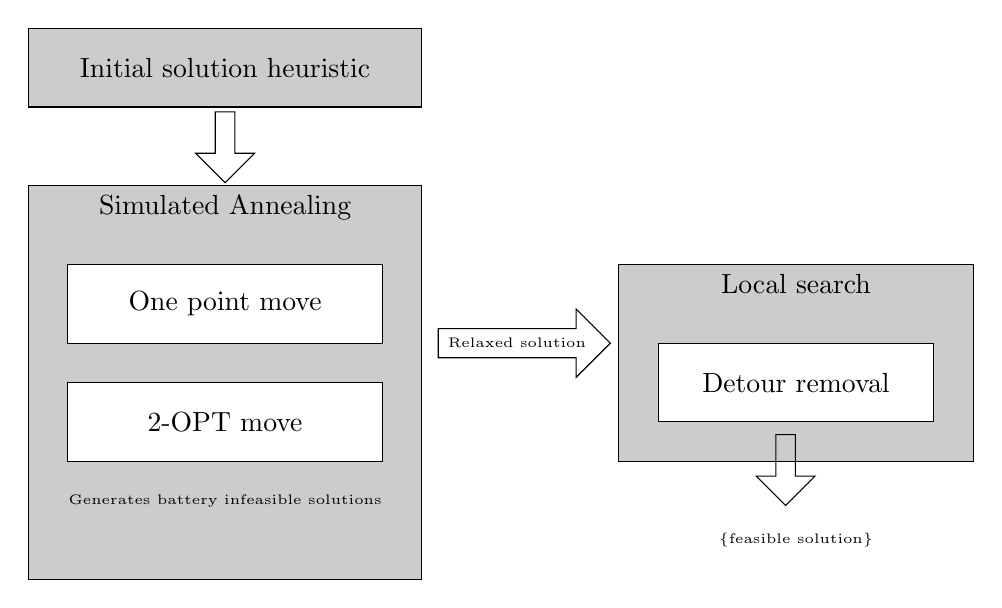
\begin{tikzpicture}
        \filldraw[fill=gray!40, draw=black] (0, 6) rectangle node {Initial solution heuristic} (5, 7);

        \filldraw[fill=gray, draw=black] (2.5, 5.55) node[draw, single arrow, minimum height=.9cm, rotate=-90] {};

        \filldraw[fill=gray!40, draw=black] (0, 0) rectangle (5, 5);
        \draw (2.5,5) node[below] {Simulated Annealing};
        \filldraw[fill=white, draw=black] (.5, 3) rectangle node {One point move} (4.5, 4);
        \filldraw[fill=white, draw=black] (.5, 1.5) rectangle node {2-OPT move} (4.5, 2.5);
        \draw (2.5, 1) node {{\tiny 
                Generates battery infeasible solutions
            }};
        \filldraw[fill=gray, draw=black] (5.2, 3) node[draw, single arrow, minimum height=.9cm, rotate=0, right] {{\tiny Relaxed solution}};

        \filldraw[fill=gray!40, draw=black] (7.5, 4) rectangle (12, 1.5);
        \draw (9.75,4) node[below] {Local search};
        \filldraw[fill=white, draw=black] (8, 2) rectangle node {Detour removal} (11.5, 3);

        \filldraw[fill=white, draw=black] (9.75, 1.45) node[draw, single arrow, minimum height=.9cm, rotate=-90, below] {};
        \draw (9.75 , .5) node {\tiny $\{\textrm{feasible solution}\}$};

    \end{tikzpicture}

\end{frame}

\begin{frame}
    \frametitle{Initial solution heuristic}
    \begin{block}{Route first, cluster second}
        \begin{itemize}
            \item Route : TSP heuristic, nearest neighbour
            \item Cluster : bin packing first fit with $\sum_j d_j / n_v$
        \end{itemize}
    \end{block}
    \begin{block}{Scheduling heuristic}
        \begin{itemize}
            \item EDD rule on each route, optimal for $1||\sum U_j$ {\tiny (here $1|r_j|\sum U_j$)}
        \end{itemize}
    \end{block}
    \begin{exampleblock}{Idea}
        We end up with roughly coherent routes in which we minimize the number of tardy jobs \textit{without the release date constraint}.
    \end{exampleblock}
\end{frame}

\begin{frame}
    \frametitle{Simulated Annealing with VNS}
    \begin{block}{Two neighbourhoods}
        \begin{itemize}
            \item One point move (both intra and inter route)\\which hopefully improves the scheduling (and optionally others)
            \item Two opt move (both intra and inter route)\\which hopefully keeps good scheduling while minimizing distance
        \end{itemize}
    \end{block}
    \begin{block}{Objective function}
        \tiny
        \begin{align*}
            \textrm{minimize }\sum_{r\in Routes} \left(
                \sum_{(i,j)\in r} d_{ij}
                + M\times (
                    overcapactitated_r
                    + overtime_r
                    + nb\_tardy\_jobs_r
                )
            \right)
        \end{align*}
    \end{block}
    $\rightarrow$ With linear cooling schedule, empirical parameters
\end{frame}

\begin{frame}
    \frametitle{Charging decisions}
    \begin{block}{Local search}
        \begin{itemize}
            \item Start with the hypothesis that we make a detour on every arc at the closest station
            \item Local Search by randomly removing detours
        \end{itemize}
    \end{block}
    \begin{block}{Objective}
        \begin{itemize}
            \item {\tiny\[
                \sum_{r\in Routes} \left( \sum_{(i,s,j)\in Detours_r} (d_{is}+d_{sj}) + M\times nb\_under\_battery\_node_r \right)
            \]}
            \item if do not have enough time to make the detour because it would make the delivery tardy, we skip this detour (thus we do not recharge) but we still count the distance it would have cost to go to the station
        \end{itemize}
    \end{block}
    \begin{exampleblock}{Idea}
        A detour which does not improve the number of under battery nodes can be removed (thus minimizing the number of detours and travelled distance)
    \end{exampleblock}
\end{frame}

\begin{frame}
    \frametitle{Critical points}
    \begin{itemize}
        \item The charging decision is a critical point since we may take a lot of time trying to charge a relaxed solution which cannot be charge
        \item Would be good to have \textit{a piori} criterias which disclaims some solutions which cannot be charged in any way
        \item Starting by assuming that the vehicle makes a detour on every arc of the route and removing them instead of assuming that the vehicles make no detour and add ones seems more efficient (experimental) but is way more costly in time
    \end{itemize}
\end{frame}

\end{document}